\CourseSection{Supporting Schedule and Technical Material}\label{app:schedule}
\Guidance{Use appendices for a detailed timeline or Gantt chart, supporting calculations, data sheets, or additional diagrams. Cite each included appendix from the body.}

\TemplateField{Insert the detailed schedule or supporting material.}

% A second appendix can be a separate file, added after this one in main.tex:
% \input{sections/12-appendix-calculations}
% Start that file with \CourseSection{Supporting Calculations}.

\CourseSection{Detailed Comparison and Deliverables Tables}\label{app:intro-tables}
Tables~\ref{tab:intro-comparison-full} and~\ref{tab:intro-deliverables-full} expand the summary tables in Section~\ref{sec:introduction}.

\begin{singlespace}
\small
\setlength{\LTcapwidth}{\linewidth}
\begin{longtable}{@{}L{0.16\linewidth} L{0.26\linewidth} L{0.28\linewidth} L{\dimexpr0.30\linewidth-6\tabcolsep\relax}@{}}
\caption{Comparison of the proposed ASCC design with existing following-cart and shot-tracking products.}\label{tab:intro-comparison-full}\\
\rowcolor{MidGray}
\TableHeader{Design consideration} & \TableHeader{Stewart Golf Q Follow \cite{stewartQFollow}} & \TableHeader{Arccos Smart Sensors with Apple Watch \cite{arccosSmartSensors,arccosAppleWatch}} & \TableHeader{Proposed ASCC design} \\
\midrule
\endfirsthead
\rowcolor{MidGray}
\TableHeader{Design consideration} & \TableHeader{Stewart Golf Q Follow \cite{stewartQFollow}} & \TableHeader{Arccos Smart Sensors with Apple Watch \cite{arccosSmartSensors,arccosAppleWatch}} & \TableHeader{Proposed ASCC design} \\
\midrule
\endhead
\bottomrule
\endfoot
\textbf{Equipment transport} & Motorized cart carries the golf bag & Separate bag-transport solution is required & Motorized cart carries the bag and the golf-assistance hardware \\
\addlinespace[3pt]
\textbf{Golfer following} & Follows a carried Bluetooth handset; also supports remote control & No powered following hardware & Tracks one golfer and maintains a specified following distance \\
\addlinespace[3pt]
\textbf{Club detection} & None & Club-mounted sensors identify the club used on detected shots & Bag-mounted reader detects tagged-club removal and return, and warns of a missing club \\
\addlinespace[3pt]
\textbf{Distance information} & Requires separate equipment & Watch shows GPS distances and recommends clubs & Cart display shows GPS distance to the green \\
\addlinespace[3pt]
\textbf{Golfer input during play} & Handset & Watch or phone & None, apart from a remote stop button \\
\end{longtable}
\end{singlespace}

\begin{singlespace}
\small
\setlength{\LTcapwidth}{\linewidth}
\begin{longtable}{@{}L{0.17\linewidth} L{0.27\linewidth} L{0.28\linewidth} L{\dimexpr0.28\linewidth-6\tabcolsep\relax}@{}}
\caption{Project deliverables, operating assumptions, and limitations.}\label{tab:intro-deliverables-full}\\
\rowcolor{MidGray}
\TableHeader{Deliverable} & \TableHeader{Included functionality} & \TableHeader{Operating assumptions / constraints} & \TableHeader{Limitations / exclusions} \\
\midrule
\endfirsthead
\rowcolor{MidGray}
\TableHeader{Deliverable} & \TableHeader{Included functionality} & \TableHeader{Operating assumptions / constraints} & \TableHeader{Limitations / exclusions} \\
\midrule
\endhead
\bottomrule
\endfoot
\textbf{Following-cart subsystem} & Powered transport, one-golfer following, obstacle stopping, remote safety stop & Dry grass; defined terrain and speed limits; golfer detectable by the tracking system & No independent course navigation; restricted terrain capability \\
\addlinespace[3pt]
\textbf{Smart-bag subsystem} & Tagged-club identification, removal/return detection, club inventory, missing-club warning & One bag of tagged clubs; reliable reads within the defined bag configuration & Does not detect whether a removed club was used for a shot \\
\addlinespace[3pt]
\textbf{Distance display} & GPS distance to the green on an outward-facing display, with no golfer input & Usable GPS; green coordinates loaded beforehand for the test site & Measured from the cart, not the ball; subject to GPS error \\
\addlinespace[3pt]
\textbf{Integrated powered prototype} & One working cart demonstrated with all three core subsystems & Battery sized for the specified demonstration; dry-weather testing & Waterproofing and full 18-hole endurance excluded \\
\addlinespace[3pt]
\textbf{Extensions (not committed)} & Shot-distance logging from club events, player club history and club recommendation, voice or button interaction & Attempted only after the core deliverables are verified & Not part of the success criteria \\
\end{longtable}
\end{singlespace}

\CourseSection{Detailed Safety Hazards and Project Risks}\label{app:risks}
Figure~\ref{fig:safety-hazards} is the bow-tie diagram for loss of control of the cart, and Table~\ref{tab:risks-full} expands the summary in Table~\ref{tab:risks}.

\begin{figure}[H]
\centering
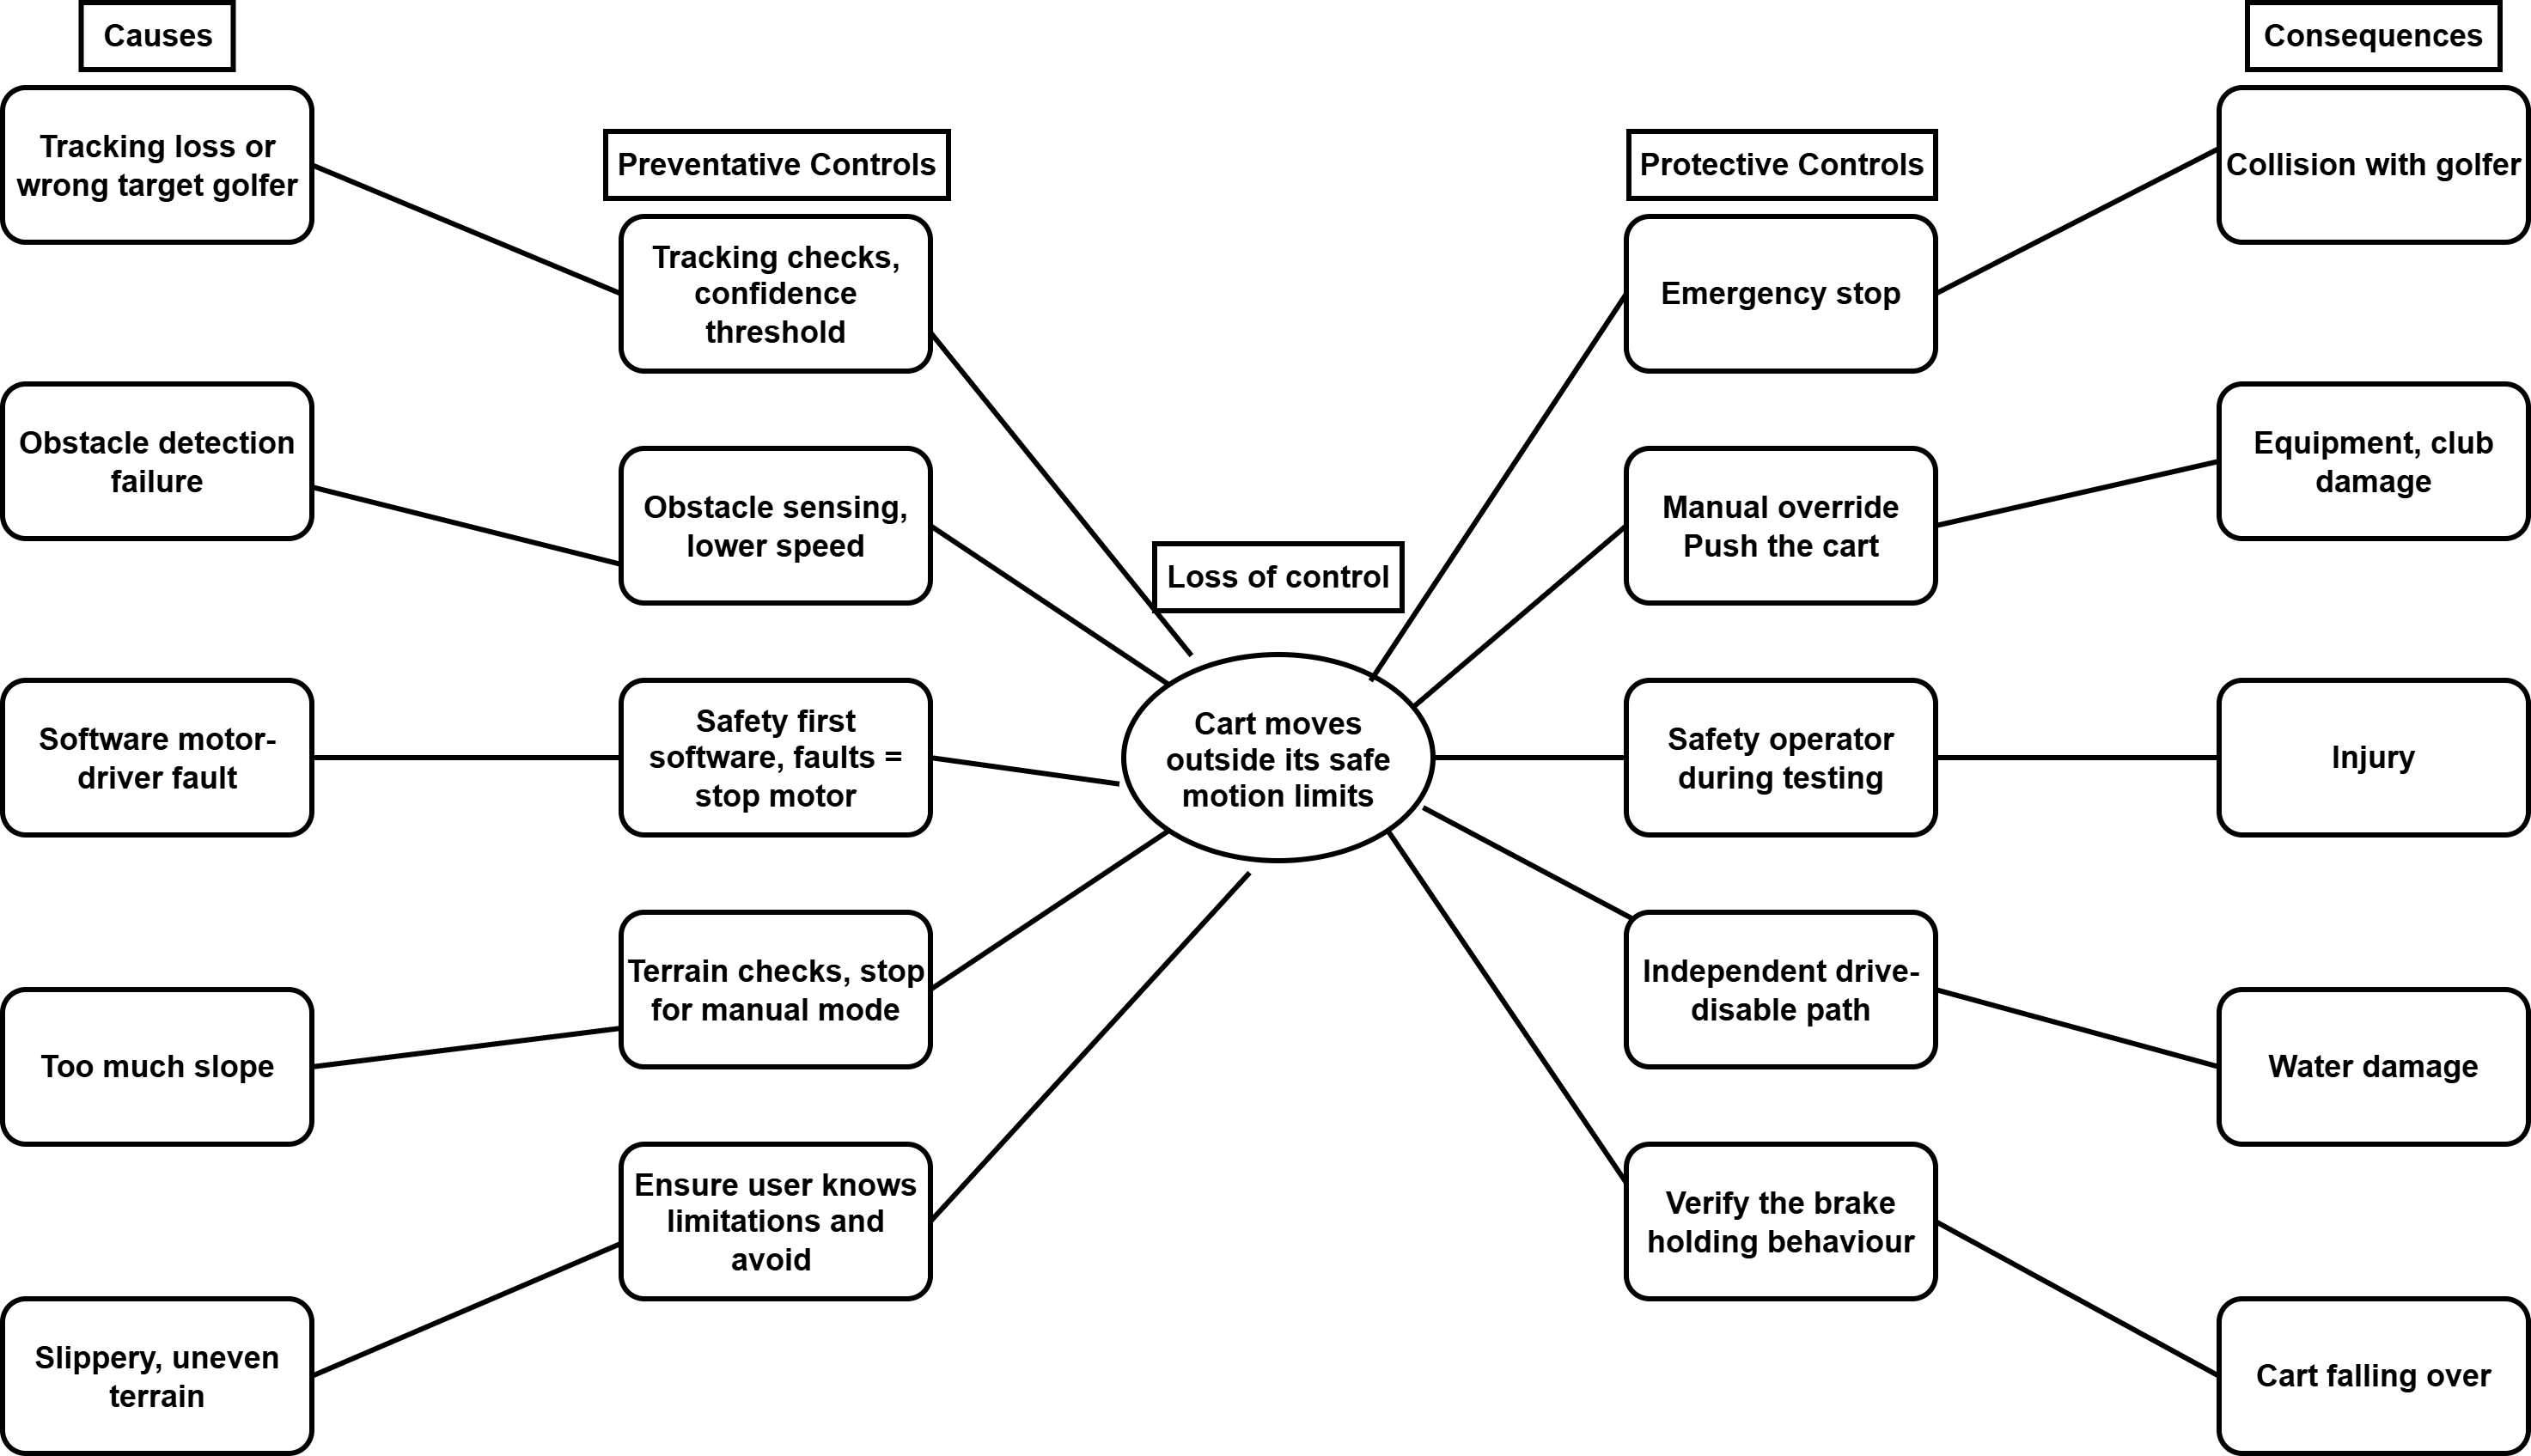
\includegraphics[width=\linewidth]{figures/safety-hazards.png}
\caption{Bow-tie diagram for loss of control of the cart, showing causes and preventative controls on the left and protective controls and consequences on the right.}
\label{fig:safety-hazards}
\end{figure}

\begin{singlespace}
\small
\setlength{\LTcapwidth}{\linewidth}
\begin{longtable}{@{}L{0.09\linewidth} L{0.25\linewidth} L{0.24\linewidth} L{\dimexpr0.42\linewidth-6\tabcolsep\relax}@{}}
\caption{Safety hazards and project risks with proposed mitigations.}\label{tab:risks-full}\\
\rowcolor{MidGray}
\TableHeader{Type} & \TableHeader{Hazard / risk} & \TableHeader{Possible consequence} & \TableHeader{Proposed mitigation} \\
\midrule
\endfirsthead
\rowcolor{MidGray}
\TableHeader{Type} & \TableHeader{Hazard / risk} & \TableHeader{Possible consequence} & \TableHeader{Proposed mitigation} \\
\midrule
\endhead
\bottomrule
\endfoot
Safety & Tracking error or obstacle missed & Cart collides with a person or equipment & Limit speed; stop on tracking loss; obstacle detection; accessible emergency stop \\
\addlinespace[3pt]
Safety & Cart rolls or tips on a slope & Injury or equipment damage & Restrict terrain and payload; use a stable bag mounting; verify stopping and holding behaviour \\
\addlinespace[3pt]
Safety & Contact with wheels or drive mechanisms & Pinching or entanglement & Guard accessible moving parts; disable drive during adjustments \\
\addlinespace[3pt]
Safety & Battery fault, short circuit, or motor overload & Overheating, burns, or fire & Suitable battery protection, fuse, wiring, charger, and current limits \\
\addlinespace[3pt]
Safety & Water reaches electronics & Electrical faults or unintended behaviour & Dry-weather operation; protected electronics; stop testing if conditions deteriorate \\
\addlinespace[3pt]
Project & Club tags cannot be read reliably inside the bag & Club inventory fails to meet its accuracy target & Test the reader/tag arrangement early; simplify bag configuration or change sensing method \\
\addlinespace[3pt]
Project & GPS accuracy is insufficient & Incorrect green-distance information & Compare with reference distances; indicate unavailable data; define an achievable accuracy target \\
\addlinespace[3pt]
Project & Subsystems take too long to integrate & Incomplete MVP demonstration & Agree on interfaces early; integrate incrementally; keep red features optional \\
\end{longtable}
\end{singlespace}

\CourseSection{Detailed Test Plan}\label{app:test-plan}
Table~\ref{tab:test-plan-full} expands the summary in Table~\ref{tab:test-plan}.

\begin{singlespace}
\setlength{\LTcapwidth}{\linewidth}
\begin{longtable}{@{}L{0.18\linewidth} L{0.41\linewidth} L{\dimexpr0.41\linewidth-4\tabcolsep\relax}@{}}
\caption{Proposed tests and the specifications each one verifies.}\label{tab:test-plan-full}\\
\rowcolor{MidGray}
\TableHeader{Requirement} & \TableHeader{Proposed test} & \TableHeader{Expected evidence of success} \\
\midrule
\endfirsthead
\rowcolor{MidGray}
\TableHeader{Requirement} & \TableHeader{Proposed test} & \TableHeader{Expected evidence of success} \\
\midrule
\endhead
\bottomrule
\endfoot

IF-01, IF-04, PF-01, PF-02, PF-03, PF-05 &
\textbf{Mobility and safety.} On a controlled grass area, the cart follows a walking golfer through straight lines and turns, meets soft obstacles, loses tracking, and receives a remote emergency stop. &
Following-distance error, tracking range, and speed stay within their specified tolerances. The cart stops for every obstacle, tracking loss, and stop command, with reaction time, stop latency, and stop-link range recorded. \\
\addlinespace[3pt]

IF-03 &
\textbf{Club identification and presence.} With the bag stationary, clubs are removed and returned one at a time and several at once. &
Every bag slot reports its club as present or absent correctly. Detection delay and missed and false events are recorded. \\
\addlinespace[3pt]

IF-02, IF-05 &
\textbf{GPS and onboard display.} At outdoor reference locations with predefined green coordinates, the displayed distance is compared with the reference distance. &
Distance error stays within the specified accuracy, and the display shows the correct, readable information at each location. \\
\addlinespace[3pt]

PF-04 &
\textbf{Range.} The cart carries a loaded bag over an extended run on one charge. &
The cart covers the specified distance without recharging. \\

\end{longtable}
\end{singlespace}

\CourseSection{Resource Access by Milestone}\label{app:resources}
Table~\ref{tab:resource-access} connects the milestones in Table~\ref{tab:proposal-milestones} to the resources each one needs.

\begin{singlespace}
\setlength{\LTcapwidth}{\linewidth}
\begin{longtable}{@{}L{0.14\linewidth} L{\dimexpr0.6100000\linewidth-4.0000000\tabcolsep\relax} L{0.25\linewidth}@{}}
\caption{Resource access by milestone.}\label{tab:resource-access}\\
\rowcolor{MidGray}
\TableHeader{Milestone} & \TableHeader{Resource / source} & \TableHeader{Access date / lead time} \\
\midrule
\endfirsthead
\rowcolor{MidGray}
\TableHeader{Milestone} & \TableHeader{Resource / source} & \TableHeader{Access date / lead time} \\
\midrule
\endhead
\bottomrule
\endfoot
% Add or replace data rows below. Keep the matching column separators.
M1 & Motors, Controller, Golf Cart & Nov 1st, 2026; ASAP \\
\addlinespace[3pt]
M2 & Raspbery Pi, Ultrasonic/Lidar Sensors, & Nov 1st, 2026; ASAP \\
\addlinespace[3pt]
M3 & RFID readers/tags, User Interface Display & Dec 1st, 2026; 2-3 weeks in advance \\
\addlinespace[3pt]
M4 & Outdoor testing area & Feb 1st, 2027; 1 week in advance \\
\end{longtable}
\end{singlespace}

\CourseSection{Detailed Cost Estimate}\label{app:budget}
Table~\ref{tab:proposal-budget-full} itemizes the subsystem totals in Table~\ref{tab:proposal-budget}.

\begin{singlespace}
\setlength{\LTcapwidth}{\linewidth}
\begin{longtable}{@{}L{\dimexpr0.5300000\linewidth-6.0000000\tabcolsep\relax} C{0.09\linewidth} L{0.18\linewidth} L{0.20\linewidth}@{}}
\caption{Preliminary cost estimate (\BudgetCurrency).}\label{tab:proposal-budget-full}\\
\rowcolor{MidGray}
\TableHeader{Item / source} & \TableHeader{Qty.} & \TableHeader{Unit cost} & \TableHeader{Total} \\
\midrule
\endfirsthead
\rowcolor{MidGray}
\TableHeader{Item / source} & \TableHeader{Qty.} & \TableHeader{Unit cost} & \TableHeader{Total} \\
\midrule
\endhead
\bottomrule
\endfoot
% Add or replace data rows below. Keep the matching column separators.
Raspberry Pi 5 - 4G & 1 & Existing & 0 CAD \\
\addlinespace[3pt]
Ultrasonic Sensors & 2 & Existing & 0 CAD \\
\addlinespace[3pt]
RFID Read Tags & 2 & 10 CAD (5) & 20 CAD \\ 
\addlinespace[3pt]
Lidar Sensor & 1 & 50 CAD & 50 CAD \\
\addlinespace[3pt]
Used Motorized Golf Cart & 1 & 250 CAD & 250 CAD \\
\addlinespace[3pt]
Motor controller & 1 & 50 CAD & 50 CAD \\
\addlinespace[3pt]
Battery/Power Supply & 1 & 75 CAD & 75 CAD \\
\addlinespace[3pt]
Mounting Hardware & 1 & 30 CAD & 30 CAD \\
\addlinespace[3pt]
Wiring, Connectors, and Switches & 1 & 30 CAD & 30 CAD \\
\addlinespace[3pt]
Tax and Shipping & - & - & 75 CAD \\
\addlinespace[3pt]
Contingency & - & - & 15 CAD \\ 
\addlinespace[3pt]
\textbf{Estimated total} &  &  & 595 CAD \\

\end{longtable}
\end{singlespace}
